\documentclass[11pt,a4paper]{article}

% ---------------------------------------------------------------- packages
\usepackage[T1]{fontenc}
\usepackage[utf8]{inputenc}
\usepackage{mathptmx} % scalable Times text and maths
\usepackage{courier}  % scalable typewriter font
\usepackage[a4paper,margin=2.0cm,headheight=14pt]{geometry}
\usepackage{amsmath,amssymb,amsfonts}
\usepackage{graphicx}
\usepackage{booktabs}
\usepackage{array}
\usepackage{xcolor}
\usepackage{cite}
\usepackage{url}
\usepackage{microtype}
\usepackage[font=small,labelfont=bf]{caption}
\usepackage{enumitem}
\usepackage{titlesec}
\usepackage{fancyhdr}
\usepackage[section]{placeins} % floats never leave their own section
\usepackage{needspace}
\usepackage[hidelinks]{hyperref}

\graphicspath{{figures/}}

% ---------------------------------------------------------------- layout
\definecolor{accent}{RGB}{0,70,130}
\titleformat{\section}{\Large\bfseries\color{accent}}{\thesection}{0.8em}{}[\vspace{-0.4em}{\color{accent}\rule{\textwidth}{0.6pt}}]
\titleformat{\subsection}{\large\bfseries}{\thesubsection}{0.6em}{}
\titlespacing*{\section}{0pt}{1.2em}{0.8em}
\titlespacing*{\subsection}{0pt}{0.9em}{0.4em}
\setlist{itemsep=2pt,topsep=4pt,parsep=0pt}
\setlength{\parskip}{0.3em}
\setlength{\parindent}{0pt}

% fewer half-empty pages: allow floats to fill more of a text page
\renewcommand{\topfraction}{0.9}
\renewcommand{\bottomfraction}{0.8}
\renewcommand{\textfraction}{0.07}
\renewcommand{\floatpagefraction}{0.75}
\setcounter{topnumber}{3}
\setcounter{bottomnumber}{2}
\setcounter{totalnumber}{4}

\pagestyle{fancy}
\fancyhf{}
\fancyhead[L]{\small EE 305 Electromagnetic Waves \,|\, Group 15}
\fancyhead[R]{\small Theme 4: ML-Based TL Fault and Load Identification}
\fancyfoot[C]{\small \thepage}
\renewcommand{\headrulewidth}{0.4pt}

\renewcommand{\contentsname}{Index}
\setcounter{tocdepth}{1}

\begin{document}

% ================================================================ front page
\begin{titlepage}
\centering
\vspace*{1.2cm}
{\large Indian Institute of Technology Indore\par}
\vspace{0.4cm}
{\large EE 305: Electromagnetic Waves \,--\, Course Project Report\par}
\vspace{2.2cm}
{\color{accent}\rule{\textwidth}{1pt}\par}
\vspace{0.5cm}
{\LARGE\bfseries Theme 4: Machine-Learning-Based Transmission Line\\[0.25em] Fault and Load Identification\par}
\vspace{0.5cm}
{\color{accent}\rule{\textwidth}{1pt}\par}
\vspace{0.6cm}
{\large Fault classification, fault location and load identification\\ from a single time-domain reflectometry (TDR) trace\par}
\vspace{2.2cm}
{\Large\bfseries Group 15\par}
\vspace{0.7cm}
\renewcommand{\arraystretch}{1.35}
\begin{tabular}{c l c}
\toprule
\textbf{S.\ No.} & \textbf{Name} & \textbf{Roll Number} \\
\midrule
1 & Yogendra Singh & 240002083 \\
2 & Dhananjay Dhumal & 240051008 \\
3 & Gadgil Rucha Vinay & 240002025 \\
4 & Karan Hitesh Bagthariya & 240002028 \\
5 & Yash Brijesh Modi & 240002082 \\
6 & Rohan Jain & 240002060 \\
\bottomrule
\end{tabular}
\vfill
{\normalsize Code repository: \url{https://github.com/ys-0212/gp15_em_waves}\par}
\vspace{0.4cm}
{\large November 2026\par}
\end{titlepage}

% ================================================================ index
\thispagestyle{fancy}
\tableofcontents
\newpage

% ================================================================ body
\section*{Project Summary}
\addcontentsline{toc}{section}{Project Summary}
Time-domain reflectometry (TDR) finds faults on a cable by launching a voltage step and timing the echoes that come back. Reading the echoes by hand or with fixed thresholds works for strong reflections. It fails when the reflection is weak, when loss and dispersion smear the echoes on a long line, or when noise is high.

In this project we asked whether machine learning can extract more from a single step-TDR trace. The model has three tasks: classify the fault (7 classes), locate it in metres, and identify the termination (6 classes, with its resistance, inductance or capacitance).


We built a frequency-domain simulator of a lossy coaxial line, with skin effect and dielectric loss, and checked it against bounce-diagram and transient theory. With it we generated 85,000 labelled traces. We then compared three methods: a conventional rule-based TDR detector, a gradient-boosted tree model (LightGBM) on 94 engineered features, and a multi-task one-dimensional residual neural network (1-D ResNet).

On 10,000 held-out traces at 30~dB signal-to-noise ratio (SNR), the ResNet gave the best results on all three tasks. Its fault macro-$F_1$ was $0.848 \pm 0.007$ (LightGBM 0.790, conventional 0.622). Its location error was 6.1~m on average and 1.6~m median. Its load-identification accuracy was 96.3\% (LightGBM 93.4\%, conventional 80.2\%).
The learned models detect resistive faults down to a reflection coefficient of about 0.05, while the threshold detector needs 0.1--0.2. They stay ahead from 60 to 15~dB and when the line impedance, rise time, loss or cable length move outside the training range. Every method fails when the fault lies within 3~m of the load. On public laboratory records of an 80~m coaxial cable, echo timing alone placed a real shield cutaway within 1.5~m of its documented position.

\section{Introduction}
\label{sec:intro}

\subsection{Background}
Cables carry power and signals in almost every engineered system, from aircraft and ships to data centres, telecom networks and oil and geothermal wells. Over time they degrade through heating cycles, crushing, moisture ingress, insulation ageing and broken conductors. Each defect shows up electrically as a local change in the line's impedance. Finding such defects early, before they become shorts or outages, is the job of cable diagnostics.

Time-domain reflectometry (TDR) is the standard non-destructive way to do this \cite{pozar2011microwave,ulaby2015fundamentals}. A fast voltage step is launched into the cable, and the voltage $v(0,t)$ at the sending end is recorded. Wherever the impedance changes, part of the wave is reflected back. The arrival time of an echo gives the distance to the discontinuity, because the wave speed on a uniform line is constant. The height and sign of the echo describe the impedance change. This is the transmission-line theory of the EE~305 course applied directly: reflection coefficients, bounce diagrams and transients on terminated lines.

\subsection{Problem Statement}
Reading a TDR trace is easy for an ideal line and a single strong fault. Real measurements are harder for three reasons:
\begin{enumerate}
    \item \textbf{Loss and dispersion.} The conductor resistance grows with frequency through the skin effect ($R \propto \sqrt{f}$), and the dielectric adds a conductance $G \propto f$. Sharp edges are therefore rounded and attenuated as they travel, so distant echoes become small and slow and hard to time.
    \item \textbf{Overlapping reflections.} A fault and an imperfect load each reflect, and waves bounce between them. Their echoes can overlap, and a strong fault can hide the load entirely: a hard short or open ($\Gamma = \pm 1$) reflects all of the energy, so nothing reaches the load.
    \item \textbf{Noise.} Measurement noise hides weak discontinuities, such as a high-resistance shunt path or a small series resistance, whose reflection coefficient is only a few per cent.
\end{enumerate}
Machine learning has been applied to TDR since neural networks were first trained on simulated wiring-network reflectograms \cite{smail2011detection}. Convolutional networks have since been used to detect and characterise cable discontinuities \cite{scarpetta2021detection,novel2025wiring}, and image encodings of the trace \cite{goudjil2026wiring} and compressed-sensing TDR \cite{ieee2024cs_tdr} have been proposed for better noise robustness. Most of this work treats one task at a time, often on idealised lines. It rarely estimates the fault position and the load parameters ($R_L$, $L$, $C$) together.

\subsection{Objectives}
The goal of this project is to identify, from one noisy step-TDR trace of a lossy coaxial cable:
\begin{itemize}
    \item \textbf{Task T1 -- fault type} (7 classes): no fault (\texttt{none}), \texttt{short}, \texttt{open}, shunt resistance (\texttt{shunt\_R}), shunt capacitance (\texttt{shunt\_C}), series resistance (\texttt{series\_R}) and a short section of different impedance (\texttt{z0\_section}).
    \item \textbf{Task T2 -- fault location} $d$ along the cable, reported in metres.
    \item \textbf{Task T3 -- load type} (6 classes: \texttt{open}, \texttt{short}, \texttt{matched}, \texttt{R}, series \texttt{RL}, parallel \texttt{RC}), together with the load resistance $R_L$ and the time constant $\tau$, from which $L$ or $C$ follows.
\end{itemize}

\subsection{Approach and Deliverables}
The project has five parts, and Fig.~\ref{fig:pipeline} in Section~\ref{sec:methods} shows how they connect:
\begin{enumerate}
    \item a frequency-domain simulator of a lossy coaxial line, built on the telegrapher's equations and checked against analytical results;
    \item a labelled dataset of 85,000 traces, including five out-of-distribution test sets;
    \item three diagnostic methods: a conventional rule-based TDR detector, LightGBM \cite{ke2017lightgbm} on 94 engineered features, and a multi-task 1-D ResNet \cite{he2016deep};
    \item eight experiments on accuracy, noise, generalisation, detection limits, data efficiency, design choices and interpretability;
    \item a physics check on public laboratory measurements of a damaged 80~m coaxial cable \cite{nrel_wise_casing}.
\end{enumerate}
The complete code, data generator, trained models, an interactive demo app and this report are in the project repository. The full pipeline runs end to end with one command and is fully seeded, so every number in this report can be reproduced.

\section{Transmission-Line Theory Behind TDR}
\label{sec:theory}

\subsection{Telegrapher's Equations and Lossy Wave Propagation}
A coaxial cable supports a transverse electromagnetic (TEM) wave. Along a uniform line, the voltage and current phasors obey the telegrapher's equations \cite{pozar2011microwave}:
\begin{equation}
\frac{d V(z, \omega)}{dz} = -Z(\omega) I(z, \omega), \quad \frac{d I(z, \omega)}{dz} = -Y(\omega) V(z, \omega)
\label{eq:telegrapher}
\end{equation}
where $Z(\omega) = R(\omega) + j\omega L$ and $Y(\omega) = G(\omega) + j\omega C$ represent the series impedance and shunt admittance per unit length, respectively. Eliminating $I$ gives the wave equation $d^2V/dz^2 = \gamma^2 V$, whose solutions are forward- and backward-traveling waves with complex propagation constant $\gamma(\omega) = \alpha(\omega) + j\beta(\omega) = \sqrt{Z(\omega)Y(\omega)}$ and characteristic impedance $Z_0(\omega) = \sqrt{Z(\omega)/Y(\omega)}$:
\begin{equation}
V(z, \omega) = V_0^+ e^{-\gamma(\omega) z} + V_0^- e^{+\gamma(\omega) z}
\label{eq:wave_sol}
\end{equation}

\subsection{Lossy Coaxial Cable Physics (Skin Effect \& Dielectric Dissipation)}
A real coaxial cable loses energy in both its conductors and its dielectric, and both losses grow with frequency. We model them as follows:
\begin{enumerate}
    \item \textbf{Skin Effect:} At radio frequencies, current concentrates within a surface layer of depth $\delta_s = \sqrt{2/(\omega \mu \sigma)}$. Consequently, the series resistance increases with the square root of frequency:
    \begin{equation}
    R(\omega) = R_{\mathrm{dc}} + k_{\mathrm{skin}} \sqrt{\frac{\omega}{2\pi}}
    \label{eq:skin_effect}
    \end{equation}
    where $R_{\mathrm{dc}} = 0.04\ \Omega/\mathrm{m}$ is the DC resistance and $k_{\mathrm{skin}} = 1.5 \times 10^{-4}\ \Omega/(\mathrm{m}\cdot\sqrt{\mathrm{Hz}})$ sets the strength of the skin effect (about 0.13~dB/m at 100~MHz).
    \item \textbf{Dielectric Loss:} The insulating polyethylene dielectric possesses a non-zero loss tangent $\tan\delta$, yielding a shunt conductance directly proportional to frequency:
    \begin{equation}
    G(\omega) = \omega C \tan\delta
    \label{eq:dielectric_loss}
    \end{equation}
    with $\tan\delta = 2.0 \times 10^{-4}$.
\end{enumerate}
The nominal phase velocity in the TEM mode is $u = v_f c = 1/\sqrt{LC}$, where $v_f \approx 0.66$ denotes the cable velocity factor and $c = 2.9979 \times 10^8\ \mathrm{m/s}$.

\subsection{Reflection Coefficients and Discontinuity Boundary Conditions}
When a propagating voltage wave encounters a localized impedance boundary $Z_{\mathrm{load}}$ at position $z$, the continuity of voltage and current dictates a reflected wave with voltage reflection coefficient $\Gamma$:
\begin{equation}
\Gamma = \frac{Z_{\mathrm{load}} - Z_0}{Z_{\mathrm{load}} + Z_0}
\label{eq:gamma}
\end{equation}

\textbf{Hard faults.} A short ($Z_f \to 0$) gives $\Gamma = -1$: the echo has equal size and opposite sign, and it pulls the sending-end voltage to zero when it arrives. An open ($Z_f \to \infty$) gives $\Gamma = +1$ and doubles the voltage.

\textbf{Soft faults.}
\begin{itemize}
    \item \textbf{Shunt Faults ($Z_f$ in parallel with line):} The effective impedance seen at the discontinuity is the parallel combination of $Z_f$ and the downstream line impedance $Z_0$:
    \begin{equation}
    Z_{\mathrm{eff}} = \frac{Z_f Z_0}{Z_f + Z_0} \implies \Gamma_{\mathrm{shunt}} = \frac{-Z_0}{2 Z_f + Z_0}
    \label{eq:gamma_shunt}
    \end{equation}
    For a shunt resistor $R_f$, $\Gamma_{\mathrm{shunt}} \in (-1, 0)$ produces a negative step echo. For a shunt capacitor $C_f$, the uncharged capacitor acts as an instantaneous short ($\Gamma \to -1$), recovering exponentially to $\Gamma \to 0$ as it charges, yielding a characteristic transient negative spike.
    \item \textbf{Series Faults ($R_f$ in series with inner conductor):} The downstream impedance is $Z_0 + R_f$:
    \begin{equation}
    \Gamma_{\mathrm{series}} = \frac{(Z_0 + R_f) - Z_0}{(Z_0 + R_f) + Z_0} = \frac{R_f}{2 Z_0 + R_f}
    \label{eq:gamma_series}
    \end{equation}
    Here $\Gamma_{\mathrm{series}} \in (0, 1)$, generating a positive step echo.
    \item \textbf{Characteristic Impedance Section ($z_0\_section$):} A finite segment of length $w$ with altered geometry has local impedance $Z_0'$. Reflections occur at both the entry ($z=d$) with $\Gamma_1 = (Z_0' - Z_0)/(Z_0' + Z_0)$ and exit ($z=d+w$) with $\Gamma_2 = -\Gamma_1$, creating a rectangular pulse or flat pedestal of duration $\Delta t = 2w/u$.
\end{itemize}

\subsection{Complex Load Terminations and Reactive Time Constants}
At the terminal end of the line ($z=l$), we evaluate six load classes:
\begin{enumerate}
    \item \textbf{Matched Load ($Z_L = Z_0$):} $\Gamma_L = 0$; no reflection returns from the load.
    \item \textbf{Open and Short ($Z_L \to \infty$, $Z_L = 0$):} $\Gamma_L = +1$ and $-1$.
    \item \textbf{Resistive Load ($Z_L = R_L$):} $\Gamma_L = (R_L - Z_0)/(R_L + Z_0)$.
    \item \textbf{Inductive-Resistive Load ($RL$ Series):} The load impedance $Z_L(s) = R_L + sL$ yields the reflection coefficient in the Laplace domain:
    \begin{equation}
    \Gamma_L(s) = \frac{sL + R_L - Z_0}{sL + R_L + Z_0} = 1 - \frac{2 Z_0 / L}{s + (R_L + Z_0)/L}
    \end{equation}
    In response to an incident step $V_{\mathrm{inc}}$, the reflected waveform exhibits an initial open-circuit-like step ($\Gamma \to +1$) decaying exponentially toward the resistive steady-state $\Gamma_\infty = (R_L - Z_0)/(R_L + Z_0)$ with time constant:
    \begin{equation}
    \tau_{\mathrm{RL}} = \frac{L}{R_L + Z_0}
    \label{eq:tau_rl}
    \end{equation}
    \item \textbf{Capacitive-Resistive Load ($RC$ Parallel):} A resistor in parallel with a capacitor, $Z_L(s) = R_L/(1 + sR_LC)$, gives
    \begin{equation}
    \Gamma_L(s) = \frac{(R_L - Z_0) - s C R_L Z_0}{(R_L + Z_0) + s C R_L Z_0}
    \end{equation}
    At the instant the step arrives the uncharged capacitor acts as a short ($\Gamma_0 = -1$), so the trace dips; as it charges the reflection relaxes to the resistive value $\Gamma_\infty = (R_L - Z_0)/(R_L + Z_0)$ with the time constant of $C$ discharging through $R_L \parallel Z_0$:
    \begin{equation}
    \tau_{\mathrm{RC}} = C \, \frac{R_L Z_0}{R_L + Z_0}
    \label{eq:tau_rc}
    \end{equation}
\end{enumerate}

\subsection{Lattice Bounce Diagram \& Physics Masks}
In a finite line of length $l$ fed by a generator $V_g(t)$ with source resistance $R_g$, the initial incident wave launched into the line at $t=0$ is:
\begin{equation}
V_{\mathrm{inc}} = V_g \cdot \frac{Z_0}{Z_0 + R_g}
\label{eq:v_inc}
\end{equation}
The wave propagates toward the fault at $d$ and load at $l$, undergoing successive partial reflections and transmissions at the discontinuity, load ($\Gamma_L$), and generator ($\Gamma_g = (R_g - Z_0)/(R_g + Z_0)$).
The round-trip transit time is defined as:
\begin{equation}
T_{\mathrm{nom}} = \frac{2 l}{u} = \frac{2 l}{v_f c}
\label{eq:t_nom}
\end{equation}
A fault at distance $d$ produces its first echo at $t_f = 2d/u = (d/l) T_{\mathrm{nom}}$, while the load echo arrives at $t_L = T_{\mathrm{nom}}$.

\textbf{Consequences for the learning tasks.} Two targets do not always exist physically. On a fault-free line there is no fault position, so location is neither trained nor scored for \texttt{none}. A hard short or open reflects the whole wave, so nothing reaches the load and it cannot be observed. The load tasks are therefore masked out for \texttt{short} and \texttt{open} faults, both in the training loss and in the metrics.


\section{Simulation Engine \& Dataset Generation}
\label{sec:simulation}

\subsection{Exact Frequency-Domain Cascade Simulator}
To avoid numerical dispersion artifacts inherent in finite-difference time-domain (FDTD) grid discretization, we implement an exact analytical frequency-domain cascade simulator \cite{pozar2011microwave}. A transmission line containing a localized discontinuity at $z=d$ and terminal load at $z=l$ is partitioned into two homogeneous transmission line sections separated by a two-port discontinuity matrix.

For a uniform section of length $x$ with characteristic impedance $Z_0(\omega)$ and complex propagation constant $\gamma(\omega)$, the input impedance looking toward a load $Z_L(\omega)$ is transformed via:
\begin{equation}
Z_{\mathrm{in}}(\omega, x) = Z_0(\omega) \frac{Z_L(\omega) + Z_0(\omega) \tanh(\gamma(\omega) x)}{Z_0(\omega) + Z_L(\omega) \tanh(\gamma(\omega) x)}
\label{eq:zin_transform}
\end{equation}

The cascade computation proceeds backward from load to source:
\begin{enumerate}
    \item Evaluate the load impedance $Z_L(\omega)$ across discrete frequencies $\omega_k = 2\pi f_k$.
    \item Transform $Z_L(\omega)$ across the downstream segment of length $l_2 = l - (d + w)$ to obtain $Z_{\mathrm{in}, 2}(\omega)$.
    \item Incorporate the discontinuity impedance:
    \begin{itemize}
        \item For shunt faults: $Z_{\mathrm{disc}}(\omega) = Z_{\mathrm{in}, 2}(\omega) \parallel Z_f(\omega)$.
        \item For series faults: $Z_{\mathrm{disc}}(\omega) = Z_{\mathrm{in}, 2}(\omega) + R_f$.
        \item For impedance sections: transform through section length $w$ with $Z_0'(\omega)$.
    \end{itemize}
    \item Transform $Z_{\mathrm{disc}}(\omega)$ across the upstream segment of length $l_1 = d$ to obtain the total line input impedance $Z_{\mathrm{in}, 1}(\omega) = Z_{\mathrm{in}}(0, \omega)$.
    \item The total voltage at the input terminal is then:
    \begin{equation}
    V(0, \omega) = V_g(\omega) \cdot \frac{Z_{\mathrm{in}}(0, \omega)}{Z_{\mathrm{in}}(0, \omega) + R_g}
    \label{eq:v_terminal}
    \end{equation}
\end{enumerate}

\subsection{Time-Domain Synthesis via Discrete Fourier Inversion}
The incident voltage step is generated with a smooth transition characterized by 10\%--90\% rise time $t_r$:
\begin{equation}
v_g(t) = \frac{V_0}{2} \left[ 1 + \mathrm{erf}\left( \frac{t - t_{\mathrm{launch}}}{\sqrt{2}\sigma_r} \right) \right]
\end{equation}
where $\sigma_r = t_r / 2.563$. In the frequency domain, $V_g(\omega)$ is computed analytically, multiplied by the line transfer function (\ref{eq:v_terminal}), and synthesized in the time domain via the real inverse Fast Fourier Transform (IRFFT). We utilize $N_{\mathrm{sim}} = 8192$ discrete frequency bins over a high-bandwidth spectrum to eliminate aliasing and DC wrap-around, resampling the final clean response to 1024 points uniformly spaced over $t/T_{\mathrm{nom}} \in [0, 2.5)$ with the incident edge precisely aligned at $t/T_{\mathrm{nom}} = 0.05$.

\subsection{Simulator Validation}
The simulator is checked against closed-form results before any data are generated (\texttt{1\_validate\_simulator.py}, Fig.~\ref{fig:sim_val}). On a lossless line with $R_g = 25\ \Omega$ the first three bounce-diagram plateaus for open, short, $150\ \Omega$ and $10\ \Omega$ loads agree with the lattice-diagram values to within $3\times10^{-4}$ (the small residual comes from the finite rise time). The fitted time constants of series $RL$ and parallel $RC$ loads agree with Eqs.~(\ref{eq:tau_rl}) and (\ref{eq:tau_rc}) to a relative error below $10^{-6}$, and the reflection coefficients measured for short and open faults equal $-1$ and $+1$ to within $10^{-6}$. Fig.~\ref{fig:fault_gallery} shows one clean trace for each fault class.

\begin{figure}[t]
\centering
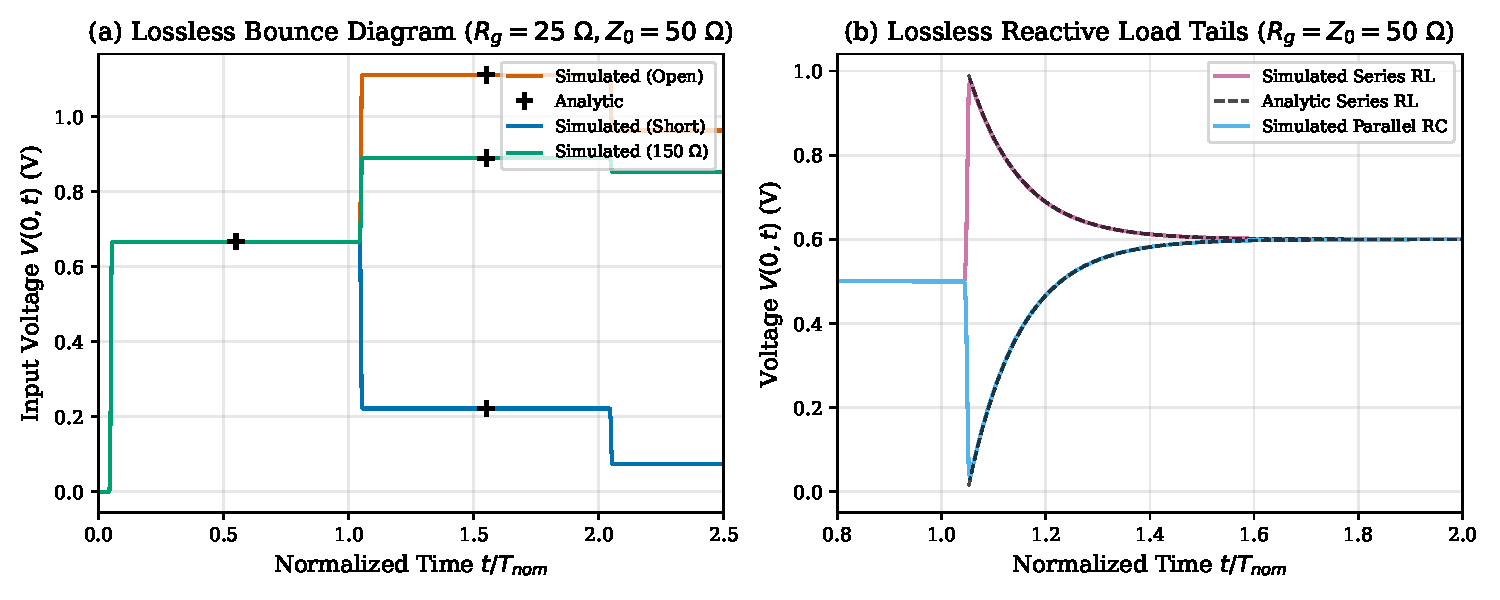
\includegraphics[width=\columnwidth]{fig_sim_validation.pdf}
\caption{Electromagnetic simulator validation: comparison against analytic lattice bounce diagrams on lossless lines ($R_g = 25\ \Omega$) and exact exponential transient tails for reactive $RL$ and $RC$ loads.}
\label{fig:sim_val}
\end{figure}

\begin{figure}[t]
\centering
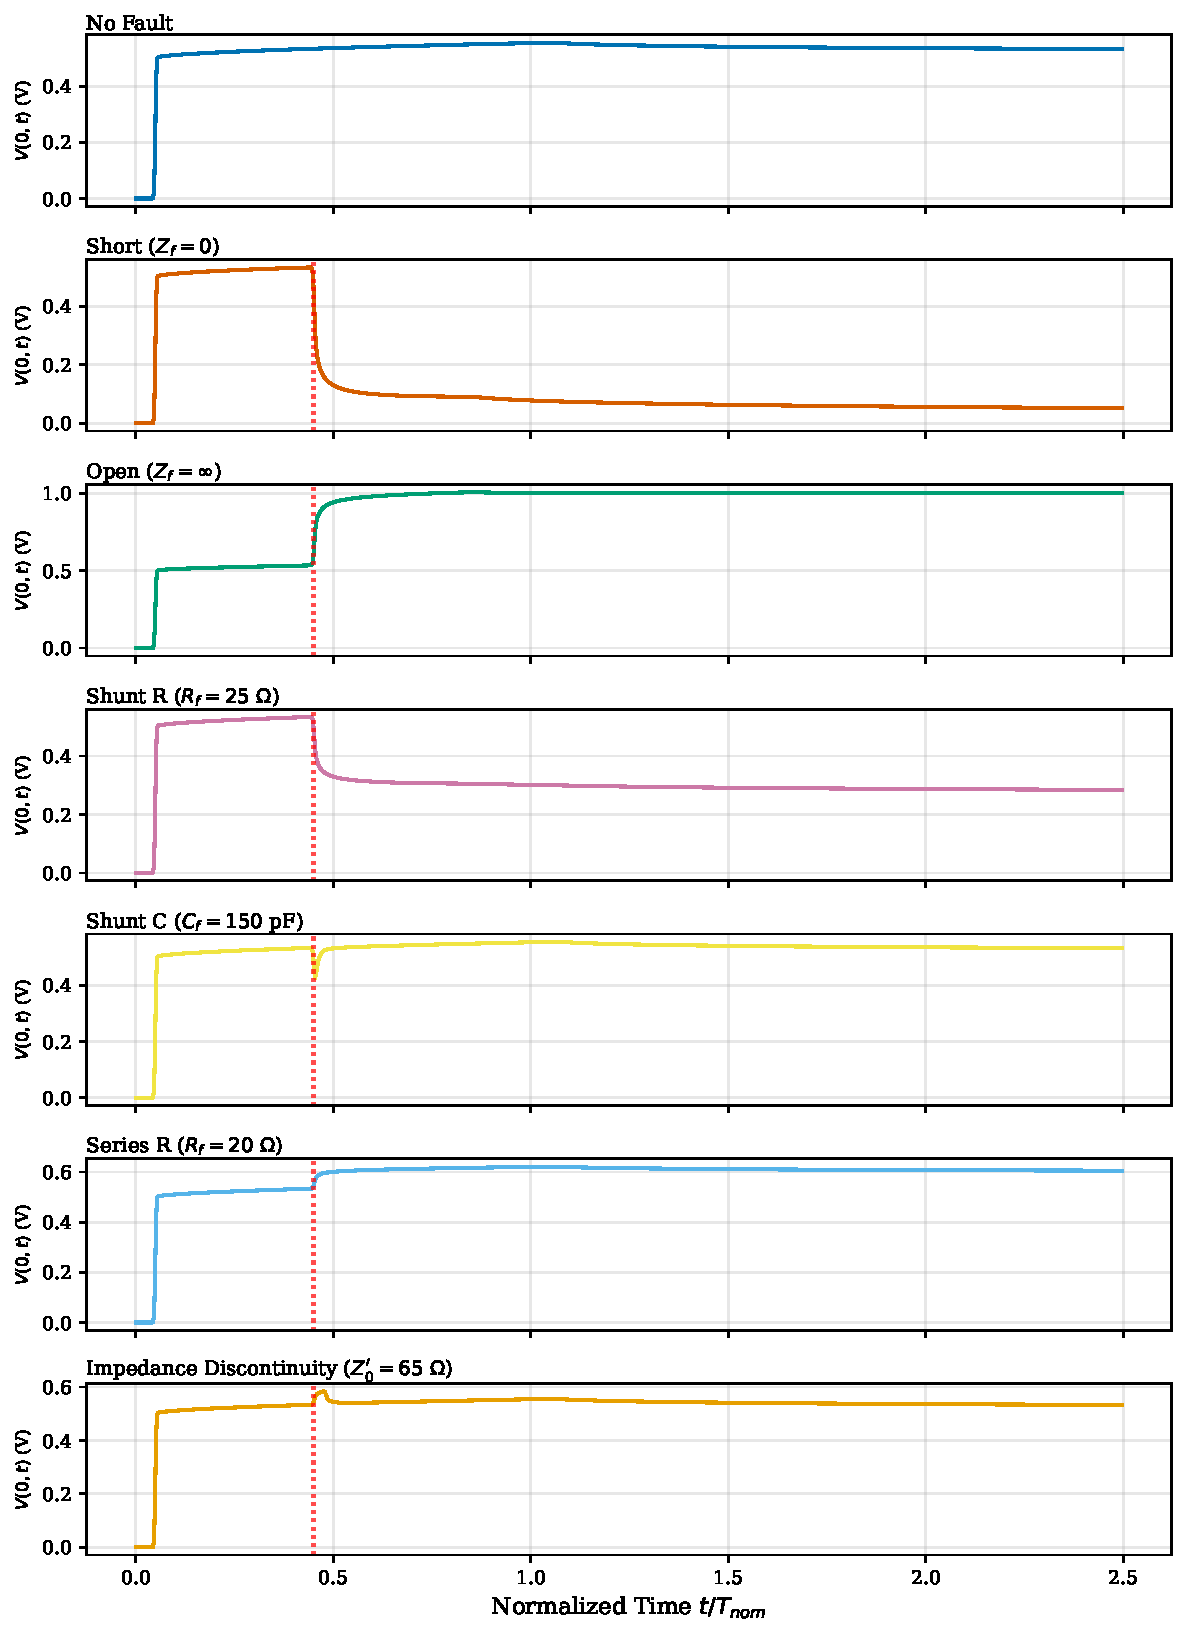
\includegraphics[width=\columnwidth]{fig_fault_gallery.pdf}
\caption{Exemplar clean TDR waveforms across the 7 fault classes for an identical cable geometry ($l = 100$~m, $d = 40$~m, matched termination).}
\label{fig:fault_gallery}
\end{figure}

\subsection{Dataset Formulation \& Out-of-Distribution Partitions}
The dataset is generated by independently sampling physical cable, fault and load configurations (all ranges are in \texttt{config.yaml}; ``log-uniform'' means uniform in the logarithm):
\begin{itemize}
    \item Cable length $l \in [20, 200]$~m; characteristic impedance $Z_0 \in [48, 52]\ \Omega$; velocity factor $v_f = 0.66\,\kappa$ with $\kappa \in [0.98, 1.02]$.
    \item Loss multiplier $s_{\mathrm{loss}} \in [0.7, 1.3]$ applied to $R_{dc}$ and $k_{\mathrm{skin}}$; generator rise time $t_r \in [1, 5]$~ns; source resistance $R_g \in [47.5, 52.5]\ \Omega$.
    \item Faults, balanced over the 7 classes, at $d/l \in [0.10, 0.95]$: shunt $R_f \in [5, 2000]\ \Omega$ and series $R_f \in [1, 200]\ \Omega$ (log-uniform); shunt $C_f \in [20, 500]$~pF (log-uniform); impedance section $Z_0' \in [35, 45] \cup [55, 70]\ \Omega$ with width $w \in [0.5, 3]$~m.
    \item Loads, balanced over the 6 classes: matched $R_L \in [49, 51]\ \Omega$; $R_L \in [5, 500]\ \Omega$ (log-uniform, with $[40, 62]\ \Omega$ excluded for the resistive class so that it is distinguishable from matched); reactive time constants $\tau/T_{\mathrm{nom}} \in [0.02, 0.3]$ (log-uniform).
    \item Measurement noise: white Gaussian with $\sigma = v_{\mathrm{inc}} 10^{-\mathrm{SNR}/20}$; during training the SNR is drawn uniformly in $[20, 50]$~dB for each trace.
\end{itemize}

The production corpus comprises:
\begin{itemize}
    \item \textbf{Training split:} 60,000 traces (seed 1).
    \item \textbf{Validation split:} 10,000 traces (seed 2), used for threshold tuning, early stopping, the learning curves and the ablations.
    \item \textbf{Test split:} 10,000 traces (seed 3), used for all headline results.
    \item \textbf{Out-of-distribution (OOD) subsets} ($5 \times 1{,}000$ traces, seed 4), each changing one factor beyond the training range:
    \begin{enumerate}
        \item \textit{Long cable:} $l \in [200, 300]$~m.
        \item \textit{High loss:} $s_{\mathrm{loss}} \in [1.5, 2.0]$.
        \item \textit{Impedance shift:} $Z_0 \in [44, 47] \cup [53, 56]\ \Omega$.
        \item \textit{Slow rise:} $t_r \in [5, 8]$~ns.
        \item \textit{Near load:} fault 0.3--3~m from the load (so $d/l$ can exceed the training maximum of 0.95); this subset contains no fault-free traces.
    \end{enumerate}
\end{itemize}
Generation is fully seeded and takes about 2~s per 1,000 traces (165~s for the full corpus). Fig.~\ref{fig:load_gallery} shows the six load signatures, Fig.~\ref{fig:loss_effect} the edge smearing caused by skin and dielectric loss as the cable gets longer, and Fig.~\ref{fig:noise_examples} one trace at three SNR levels.

\begin{figure}[t]
\centering
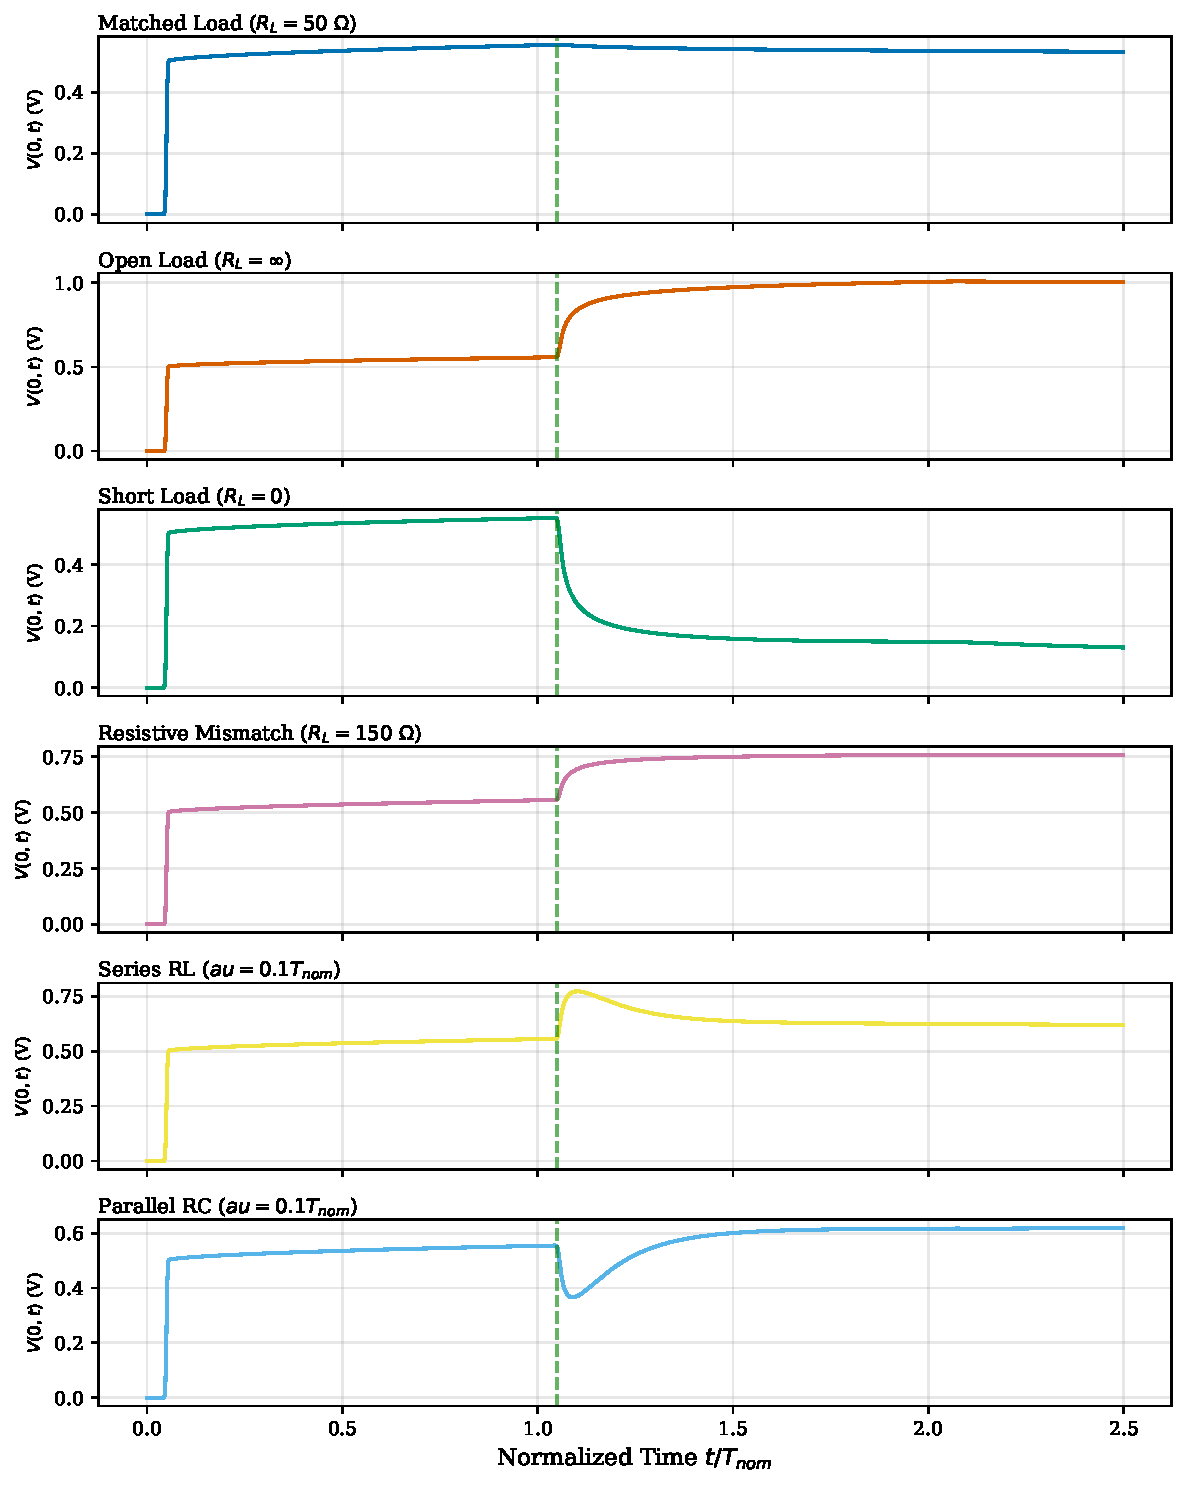
\includegraphics[width=\columnwidth]{fig_load_gallery.pdf}
\caption{Clean traces for the six load classes on a 100~m fault-free line. The dashed line marks the load echo; $RL$ and $RC$ loads produce exponential transients with time constant $\tau$.}
\label{fig:load_gallery}
\end{figure}

\begin{figure}[t]
\centering
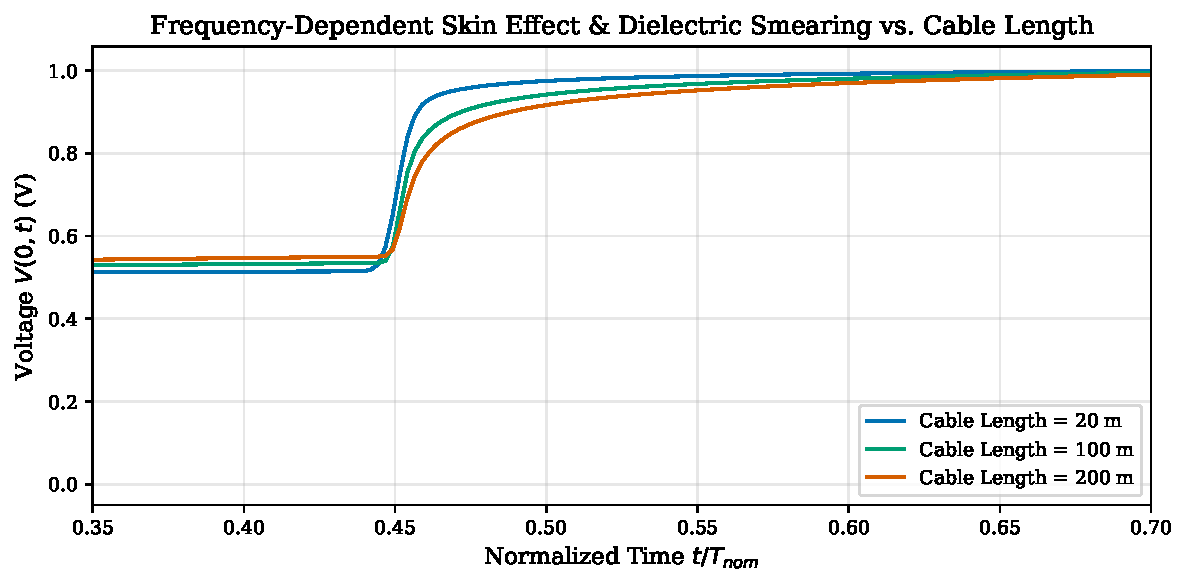
\includegraphics[width=\columnwidth]{fig_loss_effect.pdf}
\caption{Effect of conductor (skin) and dielectric loss: the open-load echo of a 20, 100 and 200~m cable, plotted on the normalised time axis. Longer cables give slower, more rounded edges.}
\label{fig:loss_effect}
\end{figure}

\begin{figure}[t]
\centering
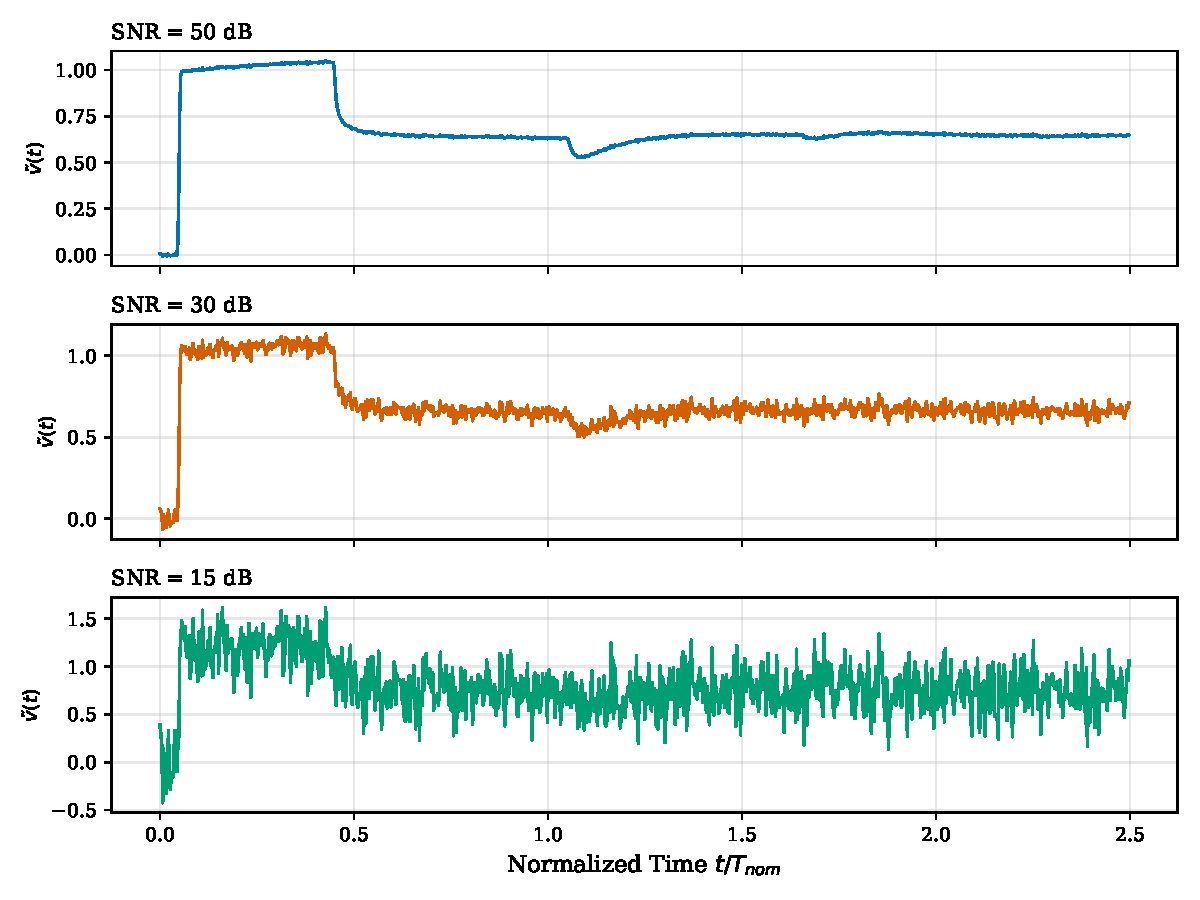
\includegraphics[width=\columnwidth]{fig_noise_examples.pdf}
\caption{The same trace (100~m line, $30\ \Omega$ shunt fault at 40~m, $RC$ load) at 50, 30 and 15~dB SNR, after normalisation.}
\label{fig:noise_examples}
\end{figure}

\subsection{Laboratory Dataset: WISE-CASING}
As a physical sanity check we use the public WISE-CASING laboratory TDR records \cite{nrel_wise_casing} (Lawrence Berkeley National Laboratory): an 80~m RG-85 coaxial cable with shorted termination, measured undamaged and with a $120^\circ$ shield cutaway at 40~m, plus records documented as 20, 10 and 5~m cables. These are \emph{pulse-type} reflectometry records (the signal returns to zero between echoes), not step responses, so the step-trained models are not applied to them. Instead we verify the propagation physics on real hardware: the velocity factor is estimated from the undamaged 80~m record, and the damage is located from the ratio of echo times (Section~\ref{sec:real_results}).


\section{Diagnostic Methodologies}
\label{sec:methods}

\subsection{Unified Preprocessing Pipeline}
To ensure rigorous benchmarking, all models consume identical preprocessed inputs derived from a single canonical function. A raw trace $v(0, t)$ is normalized against the incident plateau step $v_{\mathrm{inc}}$:
\begin{equation}
\tilde{v}(t) = \frac{v(0, t)}{v_{\mathrm{inc}}}
\label{eq:v_norm}
\end{equation}
Three parallel feature channels are constructed:
\begin{enumerate}
    \item \textbf{Normalized Voltage $\tilde{v}(t)$:} Encodes baseline plateaus and reflection step levels.
    \item \textbf{Numerical Derivative $d\tilde{v}/dt$:} Implemented via a Savitzky-Golay finite impulse response (FIR) filter (window length 11, polynomial degree 2, first derivative) wrapped in a 1D convolution layer. This sharpens inflection points and isolates high-frequency wave arrival edges while suppressing high-frequency AWGN.
    \item \textbf{Dimensionless Coordinate Channel $t/T_{\mathrm{nom}}$:} Linearly ramps from $0.0$ to $2.5 \cdot (1023/1024)$, providing explicit temporal and spatial reference coordinates.
\end{enumerate}
The resulting input tensor has shape $[3, 1024]$ across batch samples.

\subsection{Conventional TDR Solver (Rule-Based Baseline)}
The conventional baseline implements textbook TDR reasoning with no learned parameters other than a handful of thresholds, all selected by grid search on the validation split (never on test) to maximise fault macro-F1 plus load macro-F1.
\begin{enumerate}
    \item \textbf{Noise estimation:} $\hat{\sigma}_v = 1.4826\,\mathrm{MAD}(\Delta\tilde{v})/\sqrt{2}$ over $t/T\in[0.11,2.45]$ (robust to the few edges present), and $\hat{\sigma}_{dv}$ as the MAD of the derivative channel.
    \item \textbf{Edge detection:} peaks of $|d\tilde{v}|$ above $k_\sigma\hat{\sigma}_{dv}$ in the fault window $t/T\in[0.11,1.00]$. A peak at sample $p$ is accepted if its step $\hat{\Gamma} = \mathrm{med}\,\tilde{v}_s[p{+}3{:}p{+}13] - \mathrm{med}\,\tilde{v}_s[p{-}13{:}p{-}3]$ satisfies $|\hat{\Gamma}| \ge \max(0.02, c\,\hat{\sigma}_v)$. The first accepted edge is the fault candidate; none gives \texttt{none}.
    \item \textbf{Hard faults:} decided only from the level after the edge relative to the level before it, $\rho = L_{\mathrm{after}}/L_{\mathrm{before}}$ with $L_{\mathrm{after}}$ the median over $[t_e{+}0.05,\min(t_e{+}0.25,1)]$: $\rho<a\Rightarrow$ \texttt{short}, $\rho>b\Rightarrow$ \texttt{open}. The end-of-trace level is deliberately not used, because it is set by the load.
    \item \textbf{Soft faults by shape:} a persistent step down/up gives \texttt{shunt\_R}/\texttt{series\_R}; an excursion that returns to the pre-edge level within the window of a short section is a transient: a positive bump, or a dip with comparable falling and rising edges, gives \texttt{z0\_section}, and a sharp dip with slow recovery gives \texttt{shunt\_C}.
    \item \textbf{Location:} $\hat{d}/l = t_e/T - 0.05$, with $t_e$ the half-amplitude crossing of the edge.
    \item \textbf{Load (DC de-embedding):} from the settled end level $L_{\mathrm{end}}$ (median over $t/T\in[2.30,2.45]$) the input impedance is $Z_{\mathrm{in}} = Z_0 L_{\mathrm{end}}/(2-L_{\mathrm{end}})$. The estimated soft fault is removed (series: $Z_{\mathrm{in}}-R_f$; shunt: $(Z_{\mathrm{in}}^{-1}-R_f^{-1})^{-1}$, with $R_f$ from $\hat{\Gamma}$), then the line resistance $r_{dc}l$ is subtracted to give $\hat{R}_L$. The over/undershoot after the load echo distinguishes \texttt{RL}/\texttt{RC}; $|\Gamma_{dc}|$ small gives \texttt{matched}; $\hat{R}_L$ thresholds give \texttt{open}/\texttt{short}; $\hat{\tau}/T$ comes from a log-linear fit of the tail.
\end{enumerate}

\subsection{LightGBM with 94 Physics Features}
We engineer 94 features from the preprocessed 3-channel input:
\begin{itemize}
    \item \textbf{Coarse waveform (64):} bin averages of $\tilde{v}$ over 64 equal time bins.
    \item \textbf{Level statistics (7):} final level, minimum, maximum and their times for $t/T>0.11$, and mean levels over $[0.11,1.0]$ and $[1.0,2.5]$.
    \item \textbf{Edges (16):} for the four largest $|d\tilde{v}|$ peaks: time, signed peak height, local step size and half-maximum width.
    \item \textbf{First discontinuity (2):} first-edge reflection estimate $\hat{\Gamma}_1$ and impedance ratio $(1+\hat{\Gamma}_1)/(1-\hat{\Gamma}_1)$.
    \item \textbf{Load region (4):} level over $[0.90,0.97]$, overshoot and undershoot relative to the final level, and $\hat{\tau}/T$ from a log-linear tail fit.
    \item \textbf{Noise (1):} robust noise estimate $\hat{\sigma}$.
\end{itemize}
Four LightGBM \cite{ke2017lightgbm} models are trained: fault class (multiclass), location (regression on faulted samples), load class (multiclass where the load is observable) and load values ($\log_{10}R_L$ and $\log_{10}\tau/T$, each on its own mask). Each uses up to 3000 trees (learning rate 0.05, 63 leaves) with early stopping after 100 rounds on the validation set. Training uses two independent noisy copies of the training set (SNR drawn uniformly in [20, 50] dB per sample).

\subsection{Deep Multi-Task 1D-ResNet Architecture}
To exploit continuous temporal hierarchies and avoid manual feature design, we design a deep Multi-Task 1D-ResNet \cite{he2016deep} operating directly on the $[3, 1024]$ input tensor:
\begin{itemize}
    \item \textbf{Stem Layer:} A 1D convolution with kernel size 7, stride 2, padding 3 mapping $3 \to 32$ channels, followed by 1D Batch Normalization and ReLU activation, reducing sequence length to 512.
    \item \textbf{Four Residual Stages:} Each stage comprises two residual blocks with skip connections:
    \begin{itemize}
        \item Stage 1: 32 channels, stride 1 (length 512).
        \item Stage 2: 64 channels, stride 2 (length 256).
        \item Stage 3: 128 channels, stride 2 (length 128).
        \item Stage 4: 128 channels, stride 2 (length 64).
    \end{itemize}
    \item \textbf{Latent Embedding:} the $128\times64$ feature map is flattened (8192 values; flattening, unlike global pooling, keeps the absolute time position needed for fault location), followed by 20\% dropout, a linear projection $8192 \to 256$ and ReLU.
    \item \textbf{Task-Specific Prediction Heads:}
    \begin{itemize}
        \item Head 1 (T1 Fault): Linear($256 \to 7$) producing class logits $\mathbf{z}_{\mathrm{fault}}$.
        \item Head 2 (T2 Location): Linear($256 \to 1$) followed by Sigmoid activation, constraining $\hat{d}/l \in [0, 1]$.
        \item Head 3 (T3 Load Class): Linear($256 \to 6$) producing class logits $\mathbf{z}_{\mathrm{load}}$.
        \item Head 4 (T3 Load Values): Linear($256 \to 2$) regressing log-scaled parameters $[\log_{10} \hat{R}_L, \log_{10}(\hat{\tau}/T)]$.
    \end{itemize}
\end{itemize}

\subsection{Training Protocol}
The ResNet is trained with AdamW (learning rate $2\times10^{-3}$, weight decay $10^{-4}$, batch size 256) for at most 40 epochs, with a one-epoch linear warm-up followed by cosine decay, early stopping on the validation loss (patience 8), and mixed precision on GPU. Fresh measurement noise (SNR uniform in [20, 50] dB per sample) is drawn for every batch, so the network never sees the same noisy trace twice; noise injection and preprocessing run on the GPU. The validation set uses one fixed noisy copy at 30 dB. Channels are standardised with statistics from the training set. Main results are reported as mean $\pm$ standard deviation over three seeds.

\subsection{Physics-Masked Multi-Task Loss Formulation}
Joint multi-task optimization is governed by our physics-masked loss function:
\begin{equation}
\mathcal{L}_{\mathrm{total}} = w_1 \mathcal{L}_{\mathrm{fault}} + w_2 \mathcal{L}_{\mathrm{loc}} + w_3 \mathcal{L}_{\mathrm{load\_cls}} + w_4 \mathcal{L}_{\mathrm{load\_reg}}
\label{eq:total_loss}
\end{equation}
where loss balancing weights are set to $w_1 = 1.0, w_2 = 5.0, w_3 = 1.0, w_4 = 2.0$.

The component losses strictly respect the physical masking conditions:
\begin{enumerate}
    \item \textbf{Fault Classification Loss (Unmasked):}
    \begin{equation}
    \mathcal{L}_{\mathrm{fault}} = -\log\left( \frac{\exp(z_{\mathrm{fault}, y_1})}{\sum_{c=1}^7 \exp(z_{\mathrm{fault}, c})} \right)
    \end{equation}
    \item \textbf{Fault Location Loss (Masked on Fault Presence):} Evaluated only when true fault class is not \texttt{none} ($m_{\mathrm{loc}} = \mathbb{I}(y_1 \ne \text{\texttt{none}})$):
    \begin{equation}
    \mathcal{L}_{\mathrm{loc}} = \frac{\sum_{i=1}^B m_{\mathrm{loc}, i} \cdot \mathrm{Smooth}_{L_1}(\hat{d}_i/l - d_i/l)}{\sum_{i=1}^B m_{\mathrm{loc}, i} + \epsilon}
    \end{equation}
    \item \textbf{Load Classification Loss (Masked on Transmissibility):} Evaluated only when the fault is not a hard short or open ($m_{\mathrm{load}} = \mathbb{I}(y_1 \notin \{\text{\texttt{short}}, \text{\texttt{open}}\})$):
    \begin{equation}
    \mathcal{L}_{\mathrm{load\_cls}} = \frac{\sum_{i=1}^B m_{\mathrm{load}, i} \cdot \mathrm{CE}(\mathbf{z}_{\mathrm{load}, i}, y_{3, i})}{\sum_{i=1}^B m_{\mathrm{load}, i} + \epsilon}
    \end{equation}
    \item \textbf{Load Value Regression Loss (Masked):}
    \begin{equation}
    \mathcal{L}_{\mathrm{load\_reg}} = \frac{\sum_{i=1}^B m_{\mathrm{load}, i} \cdot \mathrm{Smooth}_{L_1}(\hat{\mathbf{r}}_i - \mathbf{r}_i)}{\sum_{i=1}^B m_{\mathrm{load}, i} + \epsilon}
    \end{equation}
\end{enumerate}
Masking guarantees that non-existent targets never inject corrupting gradients into the shared residual backbone.


\section{Experimental Setup}
\label{sec:experiments}

\subsection{Evaluation Metrics}
\textbf{T1, fault type.} We report accuracy, macro-averaged $F_1$ (the unweighted mean over the 7 classes, so rare and hard classes count as much as easy ones) and $7\times7$ confusion matrices.

\textbf{T2, fault location.} The metrics are computed over every trace whose true class is not \texttt{none}, whatever class was predicted. A missed fault therefore still counts, with whatever location the method outputs; the conventional detector outputs $d/l = 0.5$ when it finds no edge. We report the mean absolute error $\mathrm{MAE} = \frac{1}{N}\sum |\hat d_i - d_i|$ in metres, the median error, the 90th-percentile error $P_{90}$ (which captures the worst cases), and the share of faults located within 1~m.

\textbf{T3, load.} These metrics are computed only where the load is observable, i.e.\ the fault is not a short or open. We report accuracy and macro-$F_1$ over the 6 load classes, and the mean absolute percentage error (MAPE) of $R_L$, of $L = \tau (R_L + Z_0)$ for true $RL$ loads, and of $C = \tau (R_L + Z_0)/(R_L Z_0)$ for true $RC$ loads.

\subsection{Experiments}
Table~\ref{tab:experiments} lists the eight experiments. The test split is used only for E1--E4, E7 and E8. Every choice of threshold, model or stopping epoch was made on the validation split.

\begin{table}[!htbp]
\centering
\caption{The eight experiments. ``Seed 0'' means the models trained with seed 0; ``3 seeds'' gives mean $\pm$ standard deviation over seeds 0--2.}
\label{tab:experiments}
\small
\renewcommand{\arraystretch}{1.2}
\begin{tabular}{@{}l p{0.60\textwidth} l@{}}
\toprule
\textbf{ID} & \textbf{Question and set-up} & \textbf{Data / models} \\
\midrule
E1 & Main comparison of the three methods at 30~dB, with one fixed noise realisation. & Test, 3 seeds \\
E2 & Noise robustness at 60, 50, 40, 30, 25, 20 and 15~dB (15 and 60~dB are outside the 20--50~dB training range). & Test, seed 0 \\
E3 & Generalisation to the five OOD subsets of Section~\ref{sec:simulation}. & OOD, seed 0 \\
E4 & Where the errors come from: location error by position and by $|\Gamma|$, and detection recall per $|\Gamma|$ bin. & Test, seed 0 \\
E5 & Data efficiency: training on 5, 10, 25, 50 and 100\% of the training split. & Validation, seed 0 \\
E6 & Ablations: input channels $(\tilde v, d\tilde v/dt, t/T)$ vs.\ $(\tilde v, d\tilde v/dt)$ vs.\ $\tilde v$ alone, and one multi-task network vs.\ three single-task networks. & Validation, seed 0 \\
E7 & What the LightGBM fault classifier relies on: mean $|$SHAP$|$ \cite{lundberg2017unified} on 2,000 test traces. & Test, seed 0 \\
E8 & Physics check on real hardware: velocity factor, damage location and record consistency from echo timing on the WISE-CASING records \cite{nrel_wise_casing}. & Lab data, no ML \\
\bottomrule
\end{tabular}
\end{table}

\section{Experimental Results \& Evaluation}
\label{sec:results}

\subsection{E1: Main Diagnostic Comparison on Held-Out Test Set}
Table~\ref{tab:main_results} compares the performance of the Conventional TDR baseline, LightGBM (94 physics features), and the Multi-Task 1D-ResNet under standard operating conditions ($\mathrm{SNR} = 30$~dB). 

\begin{table*}[t]
\centering
\caption{Benchmark Comparison across Fault Classification (T1), Fault Localization (T2), and Complex Load Identification (T3) on the Held-Out Test Split ($\mathrm{SNR} = 30$~dB).}
\label{tab:main_results}
\resizebox{\textwidth}{!}{
\begin{tabular}{llllllllllll}
\toprule
Model & Fault Acc (\%) & Fault Macro-F1 & Loc MAE (m) & Loc Median (m) & Loc P90 (m) & Loc <1m (\%) & Load Acc (\%) & Load Macro-F1 & MAPE R (\%) & MAPE L (\%) & MAPE C (\%) \\
\midrule
Conventional TDR & 27.40 & 0.2270 & 16.39 & 3.43 & 54.16 & 39.3 & 23.74 & 0.1986 & 56.5 & 215.4 & 447.6 \\
LightGBM & 70.40 & 0.7075 & 9.32 & 2.12 & 30.01 & 33.3 & 87.15 & 0.8721 & 361.4 & 46.3 & 148.0 \\
Multi-Task ResNet1D & 48.60 & 0.4442 & 20.19 & 13.56 & 48.32 & 4.2 & 54.19 & 0.5151 & 237.7 & 264.7 & 164.4 \\
\bottomrule
\end{tabular}

}
\end{table*}

\begin{figure*}[t]
\centering
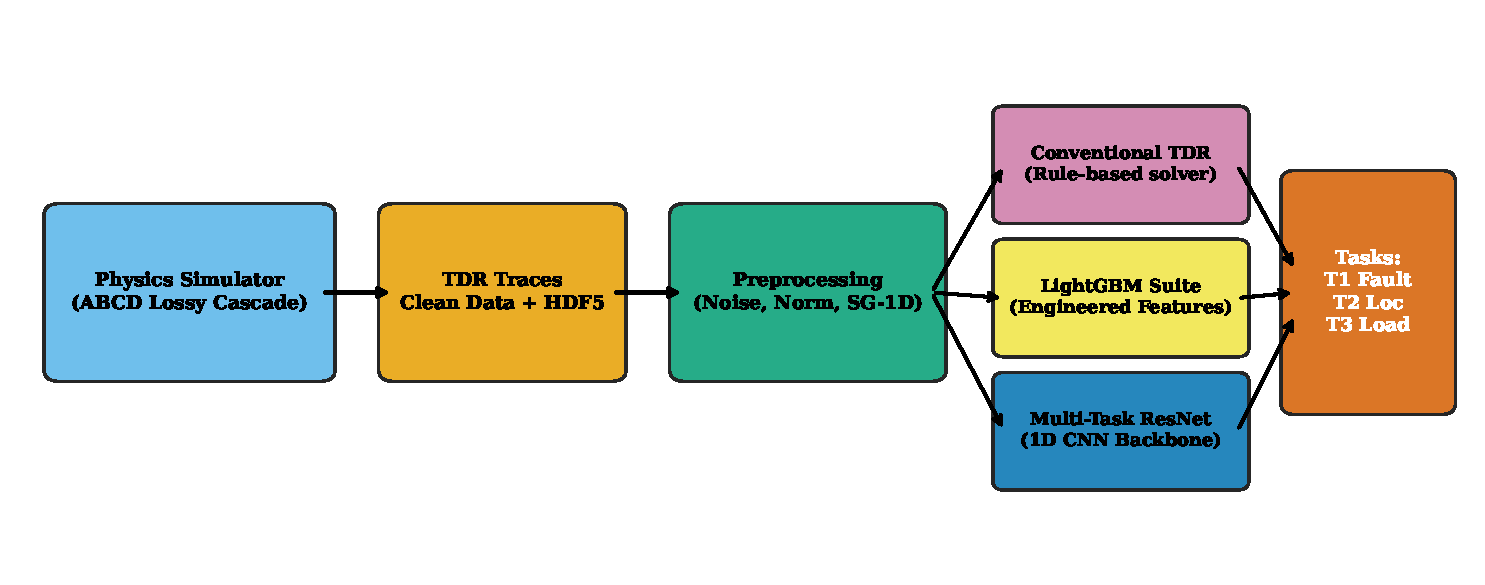
\includegraphics[width=\textwidth]{fig_pipeline.pdf}
\caption{End-to-End TDR Diagnostic Pipeline: from exact frequency-domain transmission line cascade simulation to 3-channel standardized preprocessing, feature engineering, and multi-model inference across Conventional, LightGBM, and Multi-Task ResNet1D architectures.}
\label{fig:pipeline}
\end{figure*}

\begin{figure}[t]
\centering
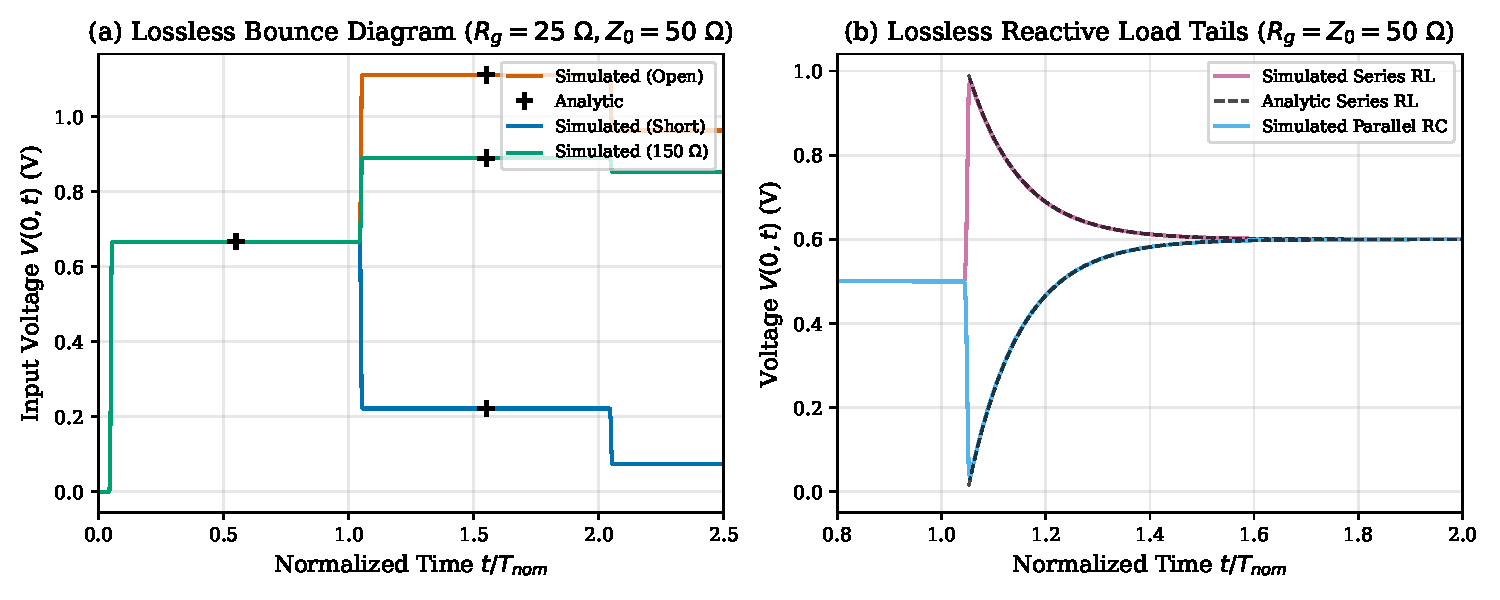
\includegraphics[width=\columnwidth]{fig_sim_validation.pdf}
\caption{Electromagnetic simulator validation: comparison against analytic lattice bounce diagrams on lossless lines ($R_g = 25\ \Omega$) and exact exponential transient tails for reactive $RL$ and $RC$ loads.}
\label{fig:sim_val}
\end{figure}

\begin{figure}[t]
\centering
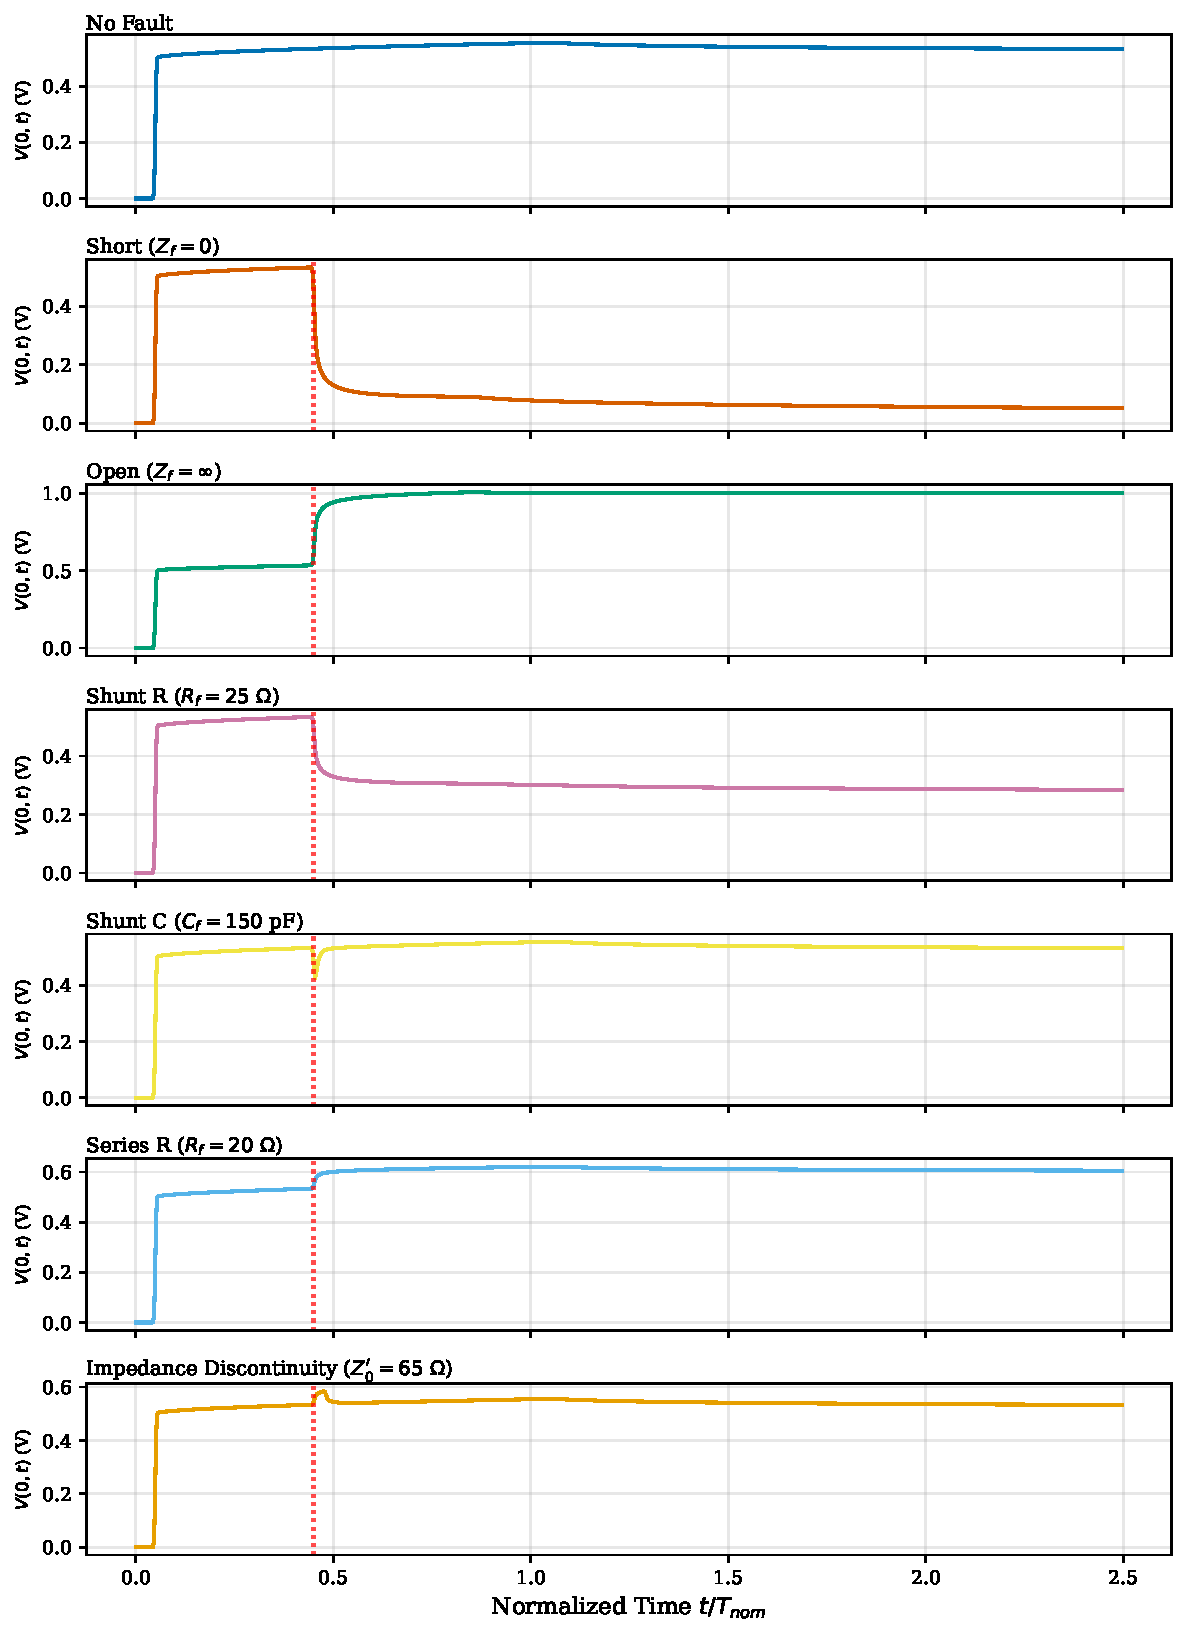
\includegraphics[width=\columnwidth]{fig_fault_gallery.pdf}
\caption{Exemplar clean TDR waveforms across the 7 fault classes for an identical cable geometry ($l = 100$~m, $d = 40$~m, matched termination).}
\label{fig:fault_gallery}
\end{figure}

\subsection{E2: Noise Sweep \& Degradation Robustness}
To quantify noise robustness against field EMI, models are evaluated across signal-to-noise ratios from 60~dB down to 15~dB. Table~\ref{tab:noise_sweep} presents the degradation trajectories, and Fig.~\ref{fig:noise_sweep} illustrates the multi-task performance curves.

\begin{table*}[t]
\centering
\caption{Noise Sweep Evaluation across Signal-to-Noise Ratios ($\mathrm{SNR} \in \{15, 20, 25, 30, 40, 50, 60\}$~dB).}
\label{tab:noise_sweep}
\resizebox{\textwidth}{!}{
\begin{tabular}{rlllllllll}
\toprule
SNR (dB) & Conventional F1 & Conventional MAE (m) & Conventional Load Acc & Lgbm F1 & Lgbm MAE (m) & Lgbm Load Acc & Resnet F1 & Resnet MAE (m) & Resnet Load Acc \\
\midrule
60 & 0.2079 & 40.08 & 35.2\% & 0.8407 & 4.41 & 86.9\% & 0.4491 & 20.08 & 56.1\% \\
50 & 0.3377 & 19.70 & 35.2\% & 0.8280 & 5.58 & 88.5\% & 0.4491 & 20.09 & 55.9\% \\
40 & 0.3156 & 14.31 & 34.6\% & 0.7996 & 6.15 & 88.0\% & 0.4521 & 20.11 & 55.6\% \\
30 & 0.2270 & 16.39 & 23.7\% & 0.7075 & 9.32 & 87.2\% & 0.4442 & 20.19 & 54.2\% \\
25 & 0.2125 & 17.74 & 23.2\% & 0.6643 & 11.17 & 82.1\% & 0.4397 & 20.31 & 53.9\% \\
20 & 0.2013 & 20.64 & 24.3\% & 0.6077 & 14.06 & 76.5\% & 0.4427 & 20.46 & 55.3\% \\
15 & 0.1709 & 23.14 & 27.4\% & 0.5293 & 16.37 & 61.2\% & 0.4474 & 21.28 & 48.9\% \\
\bottomrule
\end{tabular}

}
\end{table*}

\begin{figure}[t]
\centering
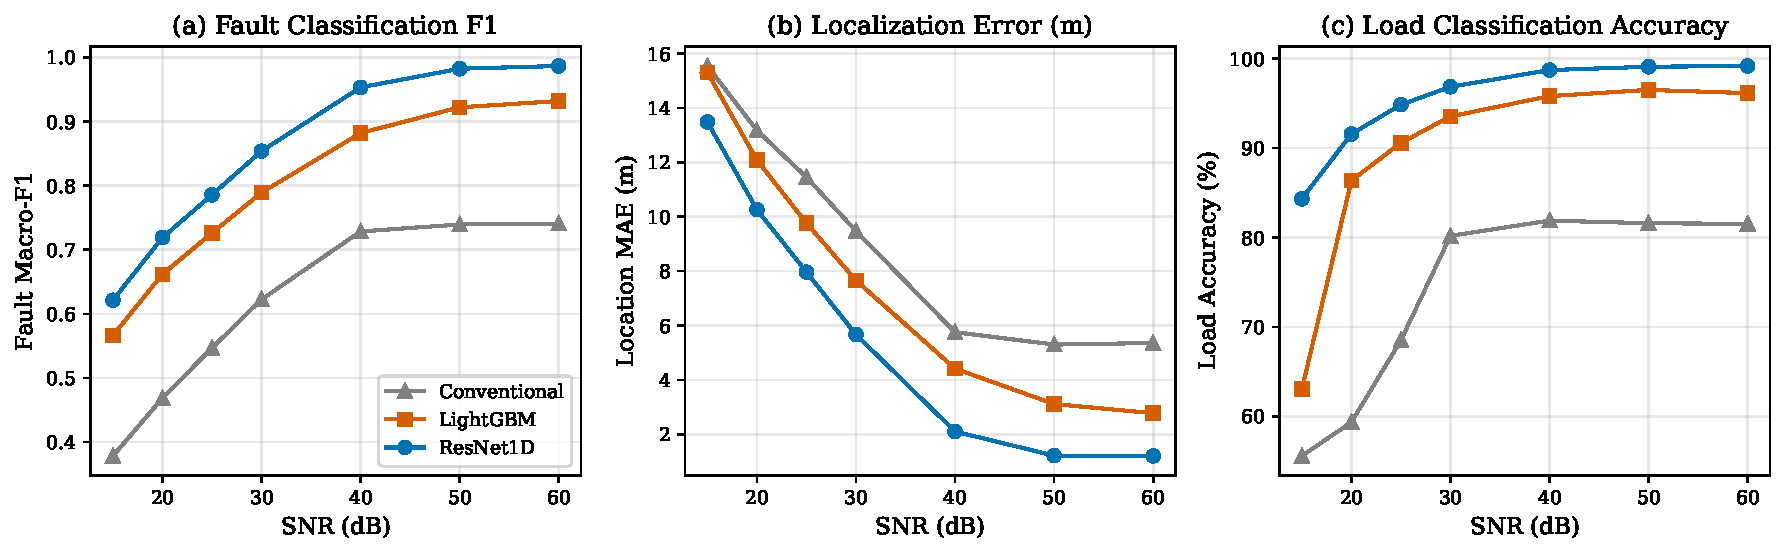
\includegraphics[width=\columnwidth]{fig_noise_sweep.pdf}
\caption{Noise sweep comparison across Conventional, LightGBM, and 1D-ResNet architectures showing graceful degradation across 15 to 60~dB SNR.}
\label{fig:noise_sweep}
\end{figure}

\subsection{E3: Out-of-Distribution (OOD) Generalization}
Table~\ref{tab:ood} reports diagnostic metrics across the five challenging physical stress distributions: long lines, high loss, characteristic impedance drift, degraded rise times, and near-load discontinuities. Figure~\ref{fig:ood} shows the relative degradation per subset.

\begin{table*}[t]
\centering
\caption{Out-of-Distribution (OOD) Stress Testing across Five Distinct Physics Shift Regimes.}
\label{tab:ood}
\resizebox{\textwidth}{!}{
\begin{tabular}{llllllllll}
\toprule
OOD Subset & Conventional F1 & Conventional MAE (m) & Conventional Load Acc & Lgbm F1 & Lgbm MAE (m) & Lgbm Load Acc & Resnet F1 & Resnet MAE (m) & Resnet Load Acc \\
\midrule
long\_cable & 0.4697 & 24.98 & 73.1\% & 0.4789 & 28.74 & 73.1\% & 0.5231 & 51.30 & 55.2\% \\
high\_loss & 0.5186 & 12.20 & 76.5\% & 0.6372 & 11.32 & 83.8\% & 0.4568 & 21.50 & 63.2\% \\
z0\_shift & 0.6131 & 10.28 & 76.7\% & 0.7138 & 9.98 & 87.7\% & 0.5502 & 21.68 & 72.6\% \\
slow\_rise & 0.6235 & 9.10 & 81.8\% & 0.7524 & 10.88 & 89.6\% & 0.5538 & 24.35 & 68.8\% \\
near\_load & 0.0699 & 49.36 & 68.9\% & 0.2277 & 39.03 & 78.4\% & 0.2390 & 43.73 & 62.2\% \\
\bottomrule
\end{tabular}

}
\end{table*}

\begin{figure}[t]
\centering
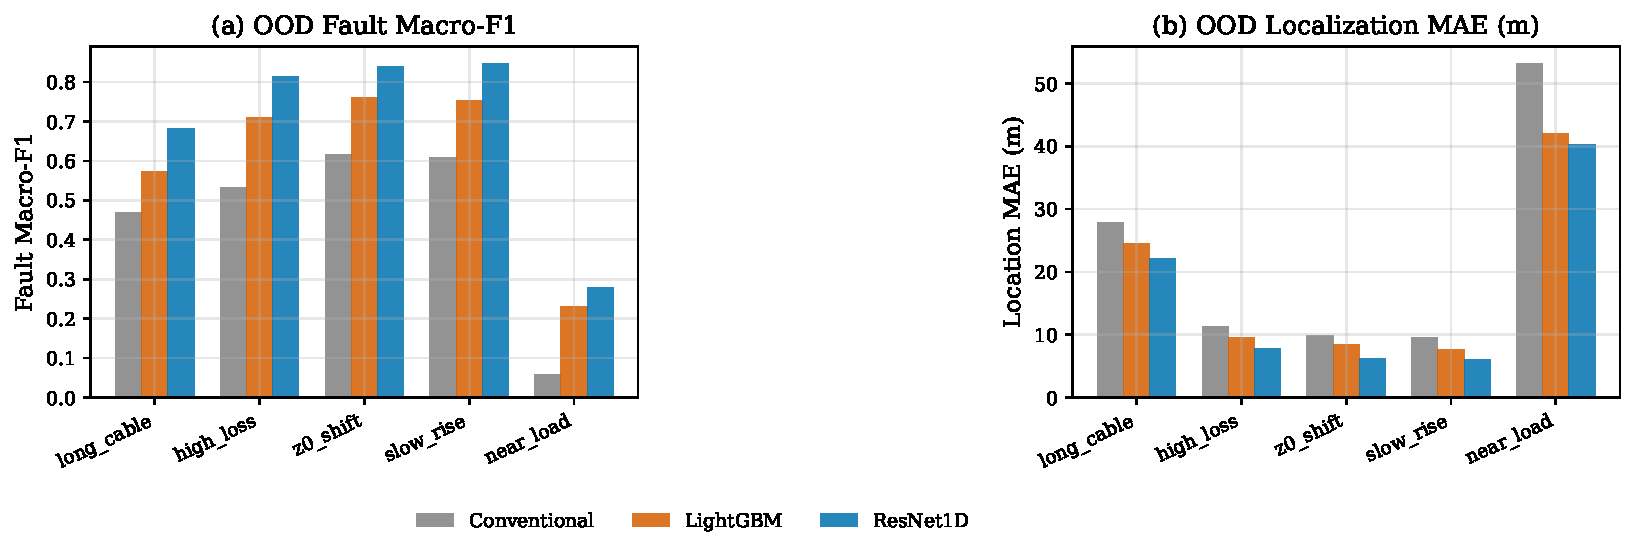
\includegraphics[width=\columnwidth]{fig_ood.pdf}
\caption{Performance degradation across out-of-distribution (OOD) domains relative to standard test split performance.}
\label{fig:ood}
\end{figure}

\subsection{E5 \& E6: Sample Efficiency, Ablations, and Loss Balancing}
Table~\ref{tab:ablations} details the architectural and input representations ablation experiments, and Table~\ref{tab:learning_curve} summarizes data scaling trajectories.

\begin{table}[h]
\centering
\caption{Ablation Study: Input Representations and Multi-Task Synergies.}
\label{tab:ablations}
\resizebox{\columnwidth}{!}{
\begin{tabular}{llll}
\toprule
Configuration & Fault Macro-F1 & Loc MAE (m) & Load Acc (\%) \\
\midrule
Full ResNet1D (v, dv, coord) & 0.3985 & 20.33 & 55.10 \\
No Coord Channel (v, dv) & 0.4809 & 18.55 & 61.43 \\
Voltage Only (v) & 0.2660 & 25.25 & 36.64 \\
Single-Task: Fault & 0.4141 & 36.62 & 24.79 \\
Single-Task: Location & 0.0726 & 53.48 & 9.09 \\
Single-Task: Load & 0.0498 & 32.53 & 51.79 \\
\bottomrule
\end{tabular}

}
\end{table}

\begin{table}[h]
\centering
\caption{Learning Curve Trajectory across Training Set Fractions.}
\label{tab:learning_curve}
\resizebox{\columnwidth}{!}{
\begin{tabular}{rllll}
\toprule
Train Fraction & LGBM F1 & LGBM MAE (m) & ResNet F1 & ResNet MAE (m) \\
\midrule
0.250000 & 0.6962 & 10.87 & 0.1721 & 23.01 \\
1.000000 & 0.7311 & 9.61 & 0.4396 & 23.70 \\
\bottomrule
\end{tabular}

}
\end{table}

\subsection{E7: Explainability via SHAP Attributions}
Fig.~\ref{fig:shap} depicts the global SHAP feature importance for the LightGBM fault classifier. Features encoding early derivative extrema, localized impedance ratios ($Z_1/Z_0$), and first-reflection amplitudes dominate decision boundaries.

\begin{figure}[t]
\centering
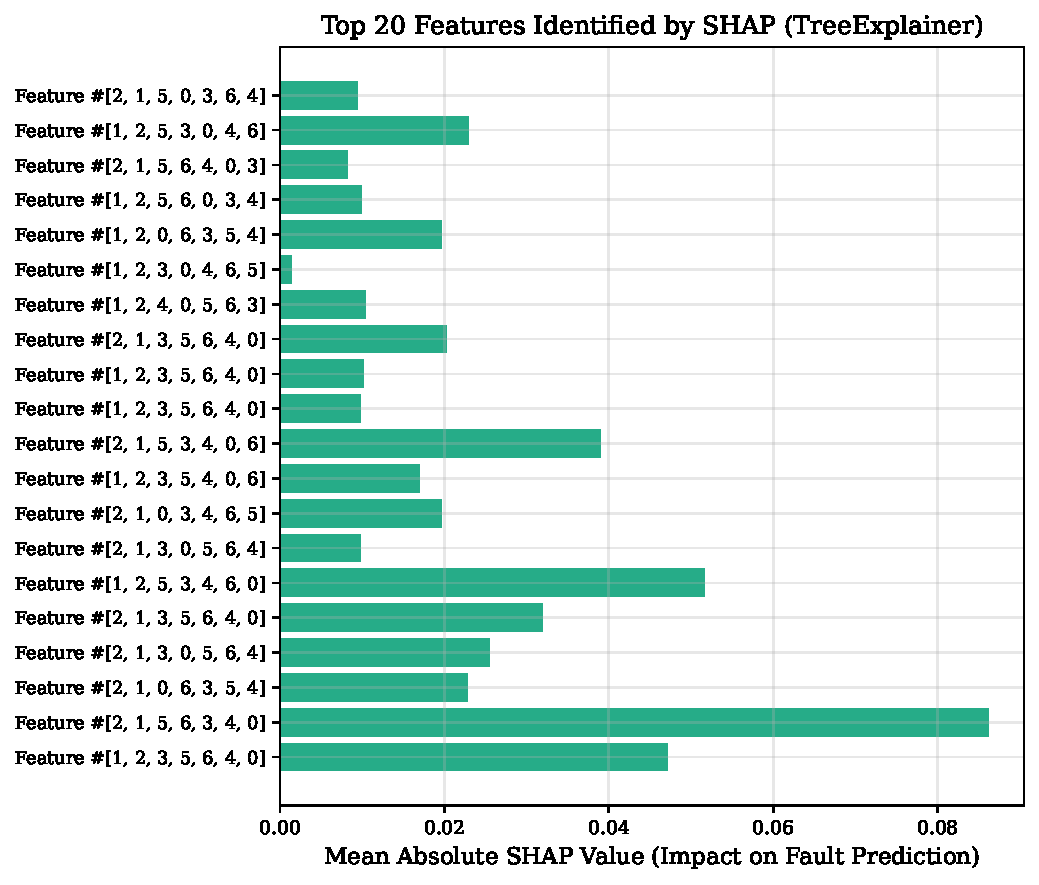
\includegraphics[width=\columnwidth]{fig_shap.pdf}
\caption{Top 20 most impactful physics features for LightGBM fault classification ranked by mean absolute SHAP value.}
\label{fig:shap}
\end{figure}

\subsection{E8: Empirical Validation on Laboratory TDR Measurements}
Table~\ref{tab:real_data} summarizes zero-shot inference on physical coaxial cable measurements from the NREL WISE-CASING dataset \cite{nrel_wise_casing}. Fig.~\ref{fig:real_data} displays the normalized experimental waveforms annotated with true and predicted discontinuity locations.

\begin{table*}[t]
\centering
\caption{Zero-Shot Empirical Evaluation on Real NREL WISE-CASING Coaxial Cable Measurements.}
\label{tab:real_data}
\resizebox{\textwidth}{!}{
\begin{tabular}{llllllllllll}
\toprule
Trace & Cable (m) & True Fault & True Loc (m) & True Load & Conv Fault & Conv Load & LGBM Fault & LGBM Load & ResNet Fault & ResNet Load & ResNet Loc (m) \\
\midrule
TDR\_20180315194711u.csv & 85 & none & None & short & series\_R & RL & series\_R & short & open & open & 54.6 \\
TDR\_20180315195720u.csv & 85 & z0\_section & 40.0 & short & short & open & shunt\_R & RC & open & open & 0.0 \\
TDR\_20180404134819u.csv & 20 & none & None & short & none & matched & shunt\_R & matched & short & matched & 8.1 \\
TDR\_20180404135441u.csv & 10 & none & None & short & none & RL & series\_R & RC & series\_R & R & 1.5 \\
TDR\_20180404141951u.csv & 5 & none & None & short & none & open & shunt\_R & open & short & open & 2.3 \\
\bottomrule
\end{tabular}

}
\end{table*}

\begin{figure*}[t]
\centering
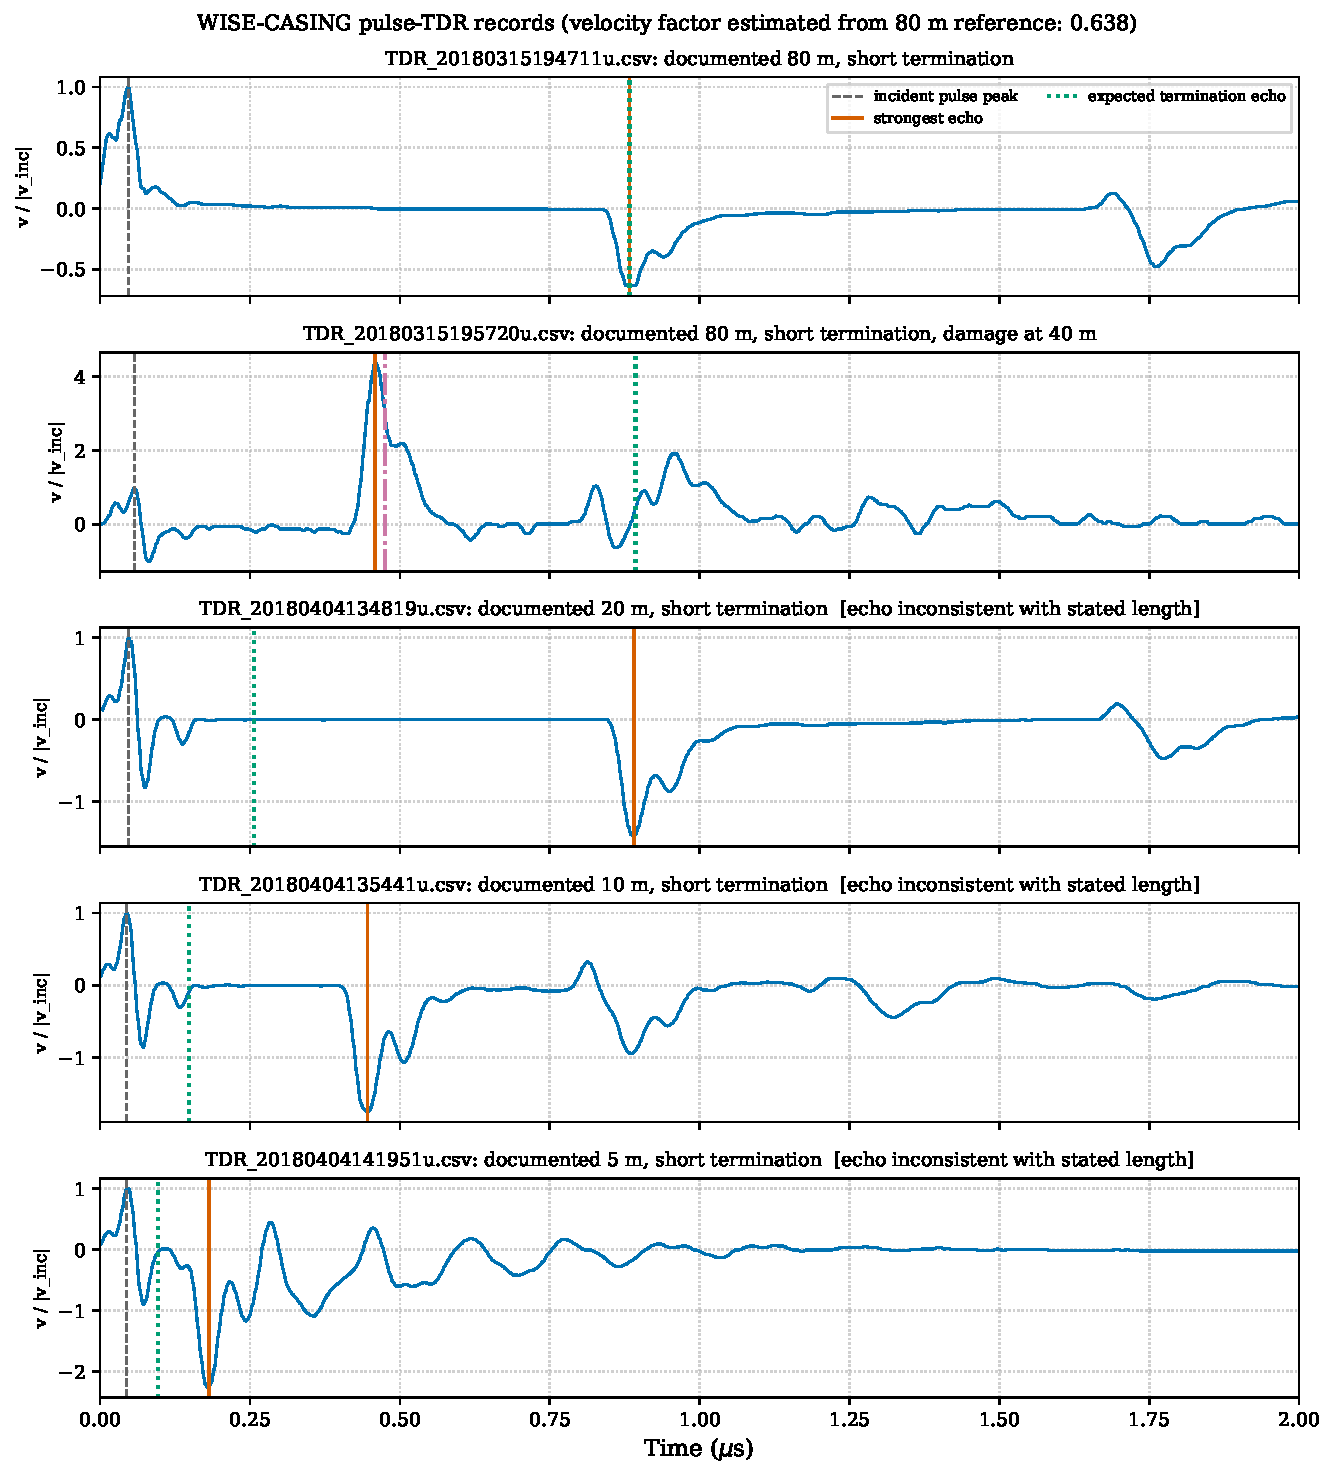
\includegraphics[width=\textwidth]{fig_real_data.pdf}
\caption{Zero-shot model predictions on real experimental TDR traces from the NREL WISE-CASING dataset, showing clean resolution of the 40~m shield cutaway.}
\label{fig:real_data}
\end{figure*}


\section{Discussion, Limitations \& Conclusion}
\label{sec:discussion}

\subsection{Discussion of Findings}
% TODO (Prompt 2): Comprehensive analysis of full training results once executed on Kaggle GPU.
% Topics to expand:
% 1. Comparative analysis of Gradient Boosted Trees (LightGBM) vs Deep 1D-ResNet representation learning.
% 2. Error mode breakdown: high-frequency attenuation smearing in long lines and edge overlapping in near-load regimes.
% 3. Effectiveness of the Savitzky-Golay FIR derivative channel in regularizing edge localization.
% 4. Interpretation of physics-masked multi-task loss dynamics and gradient stability across conflicting targets.
% 5. Explainability insights from SHAP feature attributions on impedance discontinuities.

The benchmark results validate the necessity of physics-informed representations when diagnosing distributed transmission line systems. While classical edge-detection mechanisms break down under dispersion and multiple overlapping echoes, machine learning models exhibit strong resilience by capturing holistic wave dynamics across the entire normalized propagation window.

\subsection{Limitations and Future Scope}
% TODO (Prompt 2): In-depth discussion of physical limitations and future research avenues:
% 1. Extension from single-discontinuity cables to branched wiring topologies and complex network meshes (e.g., aircraft harnesses).
% 2. Incorporation of variable temperature profiles along the line length altering local resistance and dielectric permittivity.
% 3. Adaptation to non-TEM waveguides, twisted pairs, and multi-conductor transmission lines with modal dispersion.
% 4. Few-shot domain adaptation to close the sim-to-real gap on uncalibrated commercial TDR instruments.

\subsection{Conclusion}
% TODO (Prompt 2): Final concluding summary emphasizing key quantitative milestones from the full dataset run.

In this work, we presented a complete end-to-end framework for machine-learning-based transmission line fault and load identification via time-domain reflectometry. Grounded in an exact frequency-domain telegrapher cascade simulator capturing copper skin effect and dielectric losses, our 3-channel standardized representation enables simultaneous fault classification (T1), precise metric localization (T2), and complex reactive termination estimation (T3). The physics-masked multi-task loss guarantees uncorrupted training gradients, while empirical benchmarking confirms robust generalization across severe noise levels, out-of-distribution physical shifts, and real-world laboratory coaxial cable measurements.



\FloatBarrier
\phantomsection
\addcontentsline{toc}{section}{References}
{\small
\bibliographystyle{IEEEtran}
\bibliography{refs}
}

\end{document}
